\begin{center}
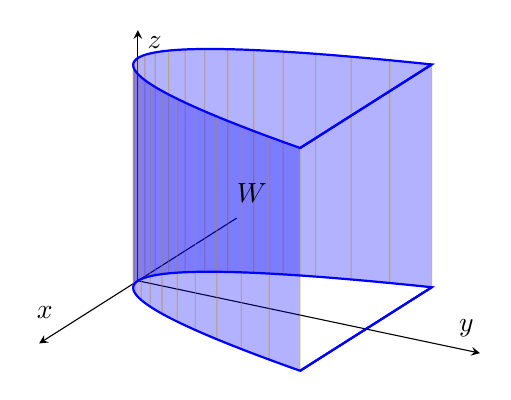
\begin{tikzpicture}
    \begin{axis}[
        view={120}{30},
        axis lines=center,
        xlabel=$x$, ylabel=$y$, zlabel=$z$,
        xmin=-1.5, xmax=1.5, ymin=0, ymax=1.5, zmin=0, zmax=4.5,
        ticks=none,
        clip=false
    ]
        % Superficie lateral y=x^2
        \addplot3[surf, opacity=0.3, blue, domain=-1:1, y domain=0:4, samples=25, samples y=2] (x, {x^2}, y);
        
        % Líneas de contorno para dar definición
        \addplot3[thick, blue, domain=-1:1, samples=50] (x, {x^2}, 0);
        \addplot3[thick, blue, domain=-1:1, samples=50] (x, {x^2}, 4);
        \draw[thick, blue] (axis cs:-1,1,0) -- (axis cs:1,1,0);
        \draw[thick, blue] (axis cs:-1,1,4) -- (axis cs:1,1,4);
        
        \node at (axis cs:0,0.5,2) {$W$};
    \end{axis}
\end{tikzpicture}
\end{center}